\section{Triển khai và thực hiện}
\subsection{Các tính năng đã triển khai}
\subsubsection{Tính năng điều khiển thiết bị thủ công}

\textbf{Mục tiêu}

Tính năng điều khiển thiết bị một cách thủ công cho phép người dùng chủ động điều chỉnh các thiết bị trong nhà kính như servo, đèn (light) và máy bơm (pump) theo ý muốn, thay vì phụ thuộc vào chế độ tự động. Điều này giúp người dùng kiểm soát tốt hơn trong những tình huống đặc biệt, hoặc khi cần can thiệp trực tiếp vào hoạt động của thiết bị.

\textbf{Quy trình hoạt động - Lấy ví dụ là điều khiển động cơ Servo}:
\begin{enumerate}
    \item Người dùng nhập lệnh điều khiển thông qua giao diện frontend, ví dụ như chọn góc mở mong muốn của servo.
    \item Frontend gửi yêu cầu POST đến API \texttt{/api/adafruit/servo} trên backend Flask, kèm theo dữ liệu góc (\texttt{angle}) do người dùng nhập.
    \begin{lstlisting}[language=Python]
@ada_fruit.route('/api/adafruit/servo', methods=['POST'])
def route_adafruit_servo():
    ...
    angle = int(data['angle'])
    return ctl_adafruit_servo(angle)
    \end{lstlisting}
    \item Flask Backend kiểm tra và xử lý dữ liệu:
    \begin{itemize}
        \item Xác minh dữ liệu đầu vào (kiểm tra có tồn tại \texttt{angle} hay không).
        \item Kiểm tra tính hợp lệ của góc: chỉ chấp nhận giá trị từ 0 đến 180 độ.
        \item Nếu dữ liệu hợp lệ, backend sử dụng thư viện \texttt{Adafruit\_IO} để gửi giá trị góc lên feed \texttt{servo} trên nền tảng Adafruit IO.
        \begin{lstlisting}[language=Python]
def route_adafruit_servo(angle):
    servo_feed = aio.feeds('servo') 
    ...
    aio.send_data(servo_feed.key, angle) 
        \end{lstlisting}
    \end{itemize}
    \item Thiết bị IoT (Yolo:Bit) đã đăng ký lắng nghe (subscribe) topic \texttt{servo} sẽ nhận được dữ liệu mới, sau đó:
    \begin{itemize}
        \item Diễn giải giá trị góc nhận được.
        \item Điều khiển servo mở theo đúng góc đã được chỉ định.
    \end{itemize}
\end{enumerate}

Cách phát triển tính năng điều khiển thủ công cho các thiết bị khác như đèn (light) và máy bơm (pump) được thực hiện tương tự như với servo:
\begin{itemize}
    \item Tạo một API riêng cho từng thiết bị, nhận giá trị điều khiển (ví dụ: ON/OFF hoặc phần trăm độ sáng).
    \item Đẩy dữ liệu tương ứng lên feed Adafruit IO đã định danh sẵn (ví dụ: \texttt{light, pump}).
    \item Thiết bị Yolo:Bit lắng nghe từng feed tương ứng và thực hiện hành động điều khiển phù hợp.
\end{itemize}

\subsubsection{Tính năng điều khiển thiết bị tự động}

\textbf{Mục tiêu}

Tính năng điều khiển thiết bị ở chế độ tự động được phát triển nhằm giúp hệ thống nhà kính có khả năng phản ứng linh hoạt và chủ động trước các điều kiện môi trường thay đổi. Thay vì yêu cầu người dùng điều khiển thủ công từng thiết bị, hệ thống sẽ tự động đưa ra quyết định kích hoạt hoặc điều chỉnh thiết bị như máy bơm nước (pump), đèn chiếu sáng (light), hoặc động cơ servo dựa trên các ngưỡng điều kiện do người dùng cài đặt trước đó.

Việc điều khiển tự động giúp tối ưu hóa hoạt động vận hành, giảm thiểu sự can thiệp thủ công và đảm bảo cây trồng luôn được chăm sóc trong điều kiện phù hợp nhất. Đây là một trong những bước quan trọng trong việc nâng cấp hệ thống nhà kính truyền thống thành một hệ thống nông nghiệp thông minh ứng dụng công nghệ IoT.

\textbf{Quy trình hoạt động - Lấy ví dụ là điều khiển máy bơm nước}

\begin{enumerate}
    \item Người dùng bật chế độ tự động cho thiết bị pump \newline
    Thông qua giao diện frontend, người dùng có thể chuyển chế độ hoạt động của thiết bị sang "automatic" bằng cách gửi một yêu cầu POST đến API \texttt{/api/mode/pump/automation}.
    \item Người dùng cấu hình các thông số tự động \newline
    Yêu cầu gửi kèm theo hai tham số chính trong phần \texttt{automatic\_options}:
    \begin{itemize}
        \item \texttt{threshold}: ngưỡng độ ẩm đất. Nếu độ ẩm đo được thấp hơn ngưỡng này, hệ thống sẽ kích hoạt pump.
        \item \texttt{duration}: khoảng thời gian (tính bằng giây) mà máy bơm sẽ hoạt động khi được kích hoạt.
    \end{itemize}

    \item Backend ghi nhận chế độ và cấu hình tự động \newline
    Flask backend lưu trạng thái chế độ hoạt động và các tham số \texttt{threshold}, \texttt{duration} vào một tệp JSON cấu hình (\texttt{IOT\_ENV}), dùng để truy xuất nhanh khi có sự kiện xảy ra.

    \item Sensor đo độ ẩm gửi dữ liệu thời gian thực lên Adafruit IO \newline
    Thiết bị cảm biến độ ẩm đất gửi giá trị đo được lên feed riêng trên nền tảng Adafruit IO.

    \item Module giám sát tự động nhận và xử lý dữ liệu (IoT Monitor and Controller)
    Một lớp giám sát mang tên \texttt{humidListener} lắng nghe dữ liệu từ feed cảm biến. Khi có dữ liệu mới, hệ thống thực hiện các bước:
    \begin{itemize}
        \item Kiểm tra xem thiết bị pump hiện đang ở chế độ \texttt{automatic}.
        \item Đối chiếu dữ liệu độ ẩm mới với ngưỡng \texttt{threshold} đã cài đặt.
        \item Nếu độ ẩm < threshold: pump được bật lên.
        \item Pump hoạt động trong đúng khoảng \texttt{duration} giây như người dùng cài đặt, sau đó được tự động tắt.
    \end{itemize}
\end{enumerate}

\textbf{Hiện thực tính năng}

1. API ghi nhận chế độ tự động và cấu hình:

\begin{lstlisting}[language=Python]
@IOT_mode.route('/api/mode/pump/automation', methods=["POST"])
def pump_automation():
    ...
    return ctl_pump_automation(automatic_options)
\end{lstlisting}

Trong đó \texttt{ctl\_pump\_automation()} sử dụng hàm \texttt{change\_mode()} để lưu lại trạng thái tự động và các tùy chọn vào hệ thống.

2. Lớp giám sát và điều khiển tự động:

\begin{lstlisting}[language=Python]
def update(self, data):
    if get_mode('pump') != 'automatic':
        return
    ...
    if float(data) < float(pump_automatic_options['threshold']):
        # Turn pump on
        ...
        time.sleep(duration)
        # Turn pump off
\end{lstlisting}

\textbf{Ghi chú về cách hoạt động các thiết bị khác}

Cách thức hoạt động tự động của light và servo được thiết kế và triển khai tương tự như với pump:
\begin{itemize}
    \item Người dùng cấu hình điều kiện kích hoạt (ví dụ: ánh sáng dưới ngưỡng sẽ bật đèn, nhiệt độ vượt ngưỡng sẽ đóng mở servo).
    \item Hệ thống theo dõi dữ liệu cảm biến liên quan theo thời gian thực.
    \item Khi điều kiện được thỏa mãn, thiết bị sẽ tự động được bật hoặc điều chỉnh trạng thái tương ứng.
    \item Sau khi thực hiện, hệ thống cập nhật lại trạng thái và tiếp tục lắng nghe vòng lặp mới.
\end{itemize}

\subsubsection{Tính năng đặt lịch điều khiển thiết bị}

\textbf{Mục tiêu}

Tính năng đặt lịch được xây dựng nhằm giúp người dùng thiết lập sẵn các thời điểm hệ thống sẽ tự động điều khiển thiết bị mà không cần can thiệp thủ công. Điều này đặc biệt hữu ích trong các tình huống lặp lại hằng ngày hoặc định kỳ, chẳng hạn như bật đèn vào mỗi sáng sớm, mở máy bơm theo chu kỳ tưới, hoặc điều chỉnh servo vào các mốc cố định. Tính năng này góp phần nâng cao tính tự động hóa và tính cá nhân hóa trong vận hành nhà kính thông minh.

\textbf{Quy trình hoạt động - Lấy ví dụ là tính năng đặt lịch cho thiết bị Light}

\begin{enumerate}
    \item Người dùng chọn đặt lịch trên giao diện web \newline
    Tại giao diện frontend, người dùng lựa chọn thiết bị (ví dụ: \texttt{light}) và mở chức năng "Lập lịch hoạt động".

    \item Hệ thống hiển thị danh sách các job đã được cài đặt trước đó \newline
    Nếu chưa có job nào, danh sách sẽ hiển thị trống. Nếu đã có, danh sách hiện đầy đủ các job đang hoạt động để người dùng chỉnh sửa hoặc xoá.

    \item Thêm job mới bằng cách nhấn dấu "+" \newline
    Khi người dùng nhấn nút "+", một modal sẽ hiển thị, cho phép cấu hình thông tin của job mới.

    \item Chọn kiểu đặt lịch (Trigger mode) \newline
    Người dùng có thể chọn giữa hai chế độ đặt lịch:
    \begin{itemize}
        \item Interval: lặp lại theo khoảng thời gian (ví dụ: mỗi 1 giờ 30 phút).
        \item Cron: lặp lại theo lịch cố định (ví dụ: 6 giờ sáng mỗi ngày).
    \end{itemize}

    \item Nhập thông tin thời gian \newline
    Tuỳ vào kiểu trigger đã chọn, người dùng sẽ được cung cấp các trường thông tin khác nhau:
    \begin{itemize}
        \item Với interval: các tùy chọn gồm \texttt{weeks}, \texttt{days}, \texttt{hours}, \texttt{minutes}, \texttt{seconds}.
        \item Với cron: các trường như \texttt{year}, \texttt{month}, \texttt{day}, \texttt{day\_of\_week}, \texttt{hour}, \texttt{minute}, \texttt{second}.
    \end{itemize}

    Ví dụ:
    \begin{itemize}
        \item \texttt{interval}: \texttt{\{ "hours": 1, "minutes": 30 \}} → lặp mỗi 1 giờ 30 phút.
        \item \texttt{cron}: \texttt{\{ "hour": 6 \}} → thực hiện lúc 6h sáng mỗi ngày.
    \end{itemize}


    \item Chọn hành động (action) và thông số \newline
    Ví dụ với thiết bị \texttt{light}, người dùng chọn cường độ ánh sáng (\texttt{intensity}) cần đặt.
    
    \item Thêm job mới \newline
    Sau khi hoàn tất cấu hình, người dùng bấm "Add Job", hệ thống sẽ lưu lại job vào bộ lập lịch và thực thi theo đúng thời gian định sẵn.
\end{enumerate}

\textbf{Hiện thực tính năng}
\begin{itemize}
    \item Backend sử dụng APScheduler để quản lý các job chạy nền.

    \item API chính để tạo job là:
    \begin{lstlisting}[language=bash]
POST /api/job/add
    \end{lstlisting}
    \item Các trường yêu cầu:
    \begin{lstlisting}[language=Python]
{
    "device_id": "light",
    "trigger": "interval" hoặc "cron",
    "trigger_options": { ... },
    "action": "set_intensity",
    "action_options": {
        "intensity": 3
    }
}
    \end{lstlisting}
    \item Tại backend, hàm \texttt{ctl\_schedule\_light\_add\_job()} sẽ:
    \begin{itemize}
        \item Xác thực dữ liệu.
        \item Thêm job mới vào APScheduler.
        \item Gọi đến \texttt{ctl\_adafruit\_light()} để gửi giá trị điều khiển lên Adafruit IO khi đến thời điểm chạy.
        \item Lưu thông tin job vào mongoDB thông qua hàm thuộc module \newline Model - \texttt{model\_schedule\_insert\_job()}.
    \end{itemize}
\end{itemize}

Cách phát triển tính năng đặt lịch cho các thiết bị pump và servo cũng được thực hiện tương tự, chỉ khác ở action và thông số cấu hình (ví dụ: độ mở của servo, thời gian bật pump).

\subsubsection{Tính năng hiển thị dữ liệu cảm biến dưới dạng đồ thị}

\textbf{Mục tiêu}

Tính năng này cho phép người dùng theo dõi dữ liệu lịch sử từ các cảm biến môi trường (độ ẩm đất, nhiệt độ, ánh sáng) một cách trực quan và dễ hiểu thông qua các biểu đồ dạng tuyến tính. Việc trực quan hóa dữ liệu giúp người dùng dễ dàng đánh giá điều kiện sinh trưởng của cây trồng trong các khung thời gian khác nhau, đồng thời hỗ trợ phân tích để đưa ra các quyết định điều chỉnh hệ thống.

\textbf{Quy trình hoạt động}
\begin{enumerate}
    \item Người dùng truy cập Dashboard \newline
    Tại giao diện người dùng, khi người dùng điều hướng đến trang thống kê (dashboard), hệ thống sẽ hiển thị ba biểu đồ tương ứng với ba loại cảm biến:
    \begin{itemize}
        \item Cảm biến ánh sáng (light-sensor)
        \item Cảm biến nhiệt độ (temperature-sensor)
        \item Cảm biến độ ẩm đất (humid-sensor)
    \end{itemize}

    \item Hiển thị mặc định theo ngày hiện tại \newline
    Khi trang dashboard được tải, hệ thống sẽ mặc định lấy dữ liệu của ngày hiện tại để hiển thị biểu đồ cho từng loại cảm biến. Các giá trị được vẽ trên biểu đồ tuyến tính theo trục thời gian (giờ:phút:giây) trên trục hoành và giá trị cảm biến trên trục tung.
    
    \item Chọn ngày xem dữ liệu với Date Picker \newline
    Người dùng có thể chọn một ngày cụ thể khác bằng cách sử dụng lịch (date picker) ở khung bên phải. Khi ngày được thay đổi, hệ thống sẽ thực hiện gọi các API tương ứng để lấy dữ liệu cảm biến của ngày đã chọn, và cập nhật lại biểu đồ theo dữ liệu mới.
\end{enumerate}
    
\textbf{Hiện thực tính năng}

\begin{itemize}
    \item Frontend (React) \newline
    Thành phần \texttt{Statistics.jsx} là giao diện chính cho dashboard thống kê. Dữ liệu được phân tách và quản lý bằng React \texttt{useState()} cho từng loại cảm biến (soilMoisture, temperature, light). Việc gọi API thực hiện thông qua thư viện \texttt{axios}.

    \item API gọi dữ liệu cảm biến \newline
    Các endpoint được gọi có dạng:
    \begin{lstlisting}[language=bash]
/api/sensor_data/<sensor_type>?year=YYYY&month=MM&date=DD
    \end{lstlisting}
    Trong đó <sensor\_type> là humid, temperature, hoặc light.

    \item Cập nhật biểu đồ khi thay đổi ngày \newline
    Thành phần \texttt{Calendar} được sử dụng để thay đổi \texttt{selectedDate}. Khi người dùng chọn ngày mới, \texttt{useEffect()} sẽ tự động kích hoạt các truy vấn dữ liệu tương ứng cho từng cảm biến và cập nhật lại dữ liệu trục hoành (\texttt{xAxis}) và trục tung (\texttt{yAxis}) của biểu đồ.
    \item Biểu đồ riêng biệt
    Ba biểu đồ được đóng gói trong ba component:
    \begin{itemize}
        \item \texttt{SoilMoistureCard}
        \item \texttt{TemperatureCard}
        \item \texttt{LightCard}
    \end{itemize}
    Mỗi component nhận dữ liệu qua props \texttt{xAxis}, \texttt{yAxis}, và \texttt{latest}, sau đó hiển thị biểu đồ trực quan cho người dùng.
\end{itemize}
    
\subsubsection{Tính năng điều khiển thiết bị thông qua AI Chatbot}

\textbf{Mục tiêu}

Phát triển hệ thống AI Chatbot thông minh có khả năng điều khiển các thiết bị IoT trong môi trường smart farm thông qua giao tiếp tự nhiên. Hệ thống cho phép người dùng tương tác bằng ngôn ngữ tự nhiên để điều khiển các thiết bị như máy bơm, đèn LED, và servo motor mà không cần phải hiểu rõ về lệnh kỹ thuật phức tạp.

\textbf{Quy trình hoạt động}
\begin{enumerate}
    \item Tiếp nhận yêu cầu từ người dùng: Người dùng nhập lệnh bằng ngôn ngữ tự nhiên qua giao diện người dùng (UI).
    \item Phân tích ngôn ngữ tự nhiên: AI Chatbot sẽ phân tích câu lệnh người dùng để trích xuất ý định (intent) và thông tin liên quan (ví dụ: thiết bị, trạng thái).
    \item Gửi yêu cầu điều khiển: Dữ liệu được gửi đến máy chủ điều khiển thiết bị (Control Server).
    \item Thực thi lệnh: Máy chủ điều khiển thực hiện yêu cầu tương ứng với các thiết bị IoT qua giao thức nội bộ.
    \item Phản hồi kết quả: Hệ thống gửi phản hồi về trạng thái hoặc kết quả thực thi về UI để hiển thị cho người dùng.
\end{enumerate}

\textbf{Hiện thực tính năng}

\begin{enumerate}
    \item Xử lý Function Calling với AI Model \newline
    Đoạn code dưới đây thực hiện việc gửi yêu cầu của người dùng đến model Gemini 2.0 Flash cùng với danh sách các function có thể gọi. Model sẽ phân tích yêu cầu và quyết định có cần gọi function nào không. Nếu có, hệ thống sẽ thực thi function đó và trả về kết quả.
    \begin{lstlisting}[language=Python]
def call_model(self, state: MessagesState):
    tools = types.Tool(function_declarations=self.tools_list)
    config = types.GenerateContentConfig(tools=[tools])
    
    response = self.client.models.generate_content(
        model="gemini-2.0-flash",
        contents=state["messages"][-1].content,
        config=config,
    )
    
    # Kiểm tra nếu có function call
    if response.candidates[0].content.parts[0].function_call:
        function_call = response.candidates[0].content.parts[0].function_call
        data = self.function_calling_excution(function_call.name, function_call.args)
        
        return {
            "messages": state["messages"] + [AIMessage(content=json.dumps(data, ensure_ascii=False))]
        }
    \end{lstlisting}

    \item Thực thi Function Calling \newline
    Khi AI model quyết định gọi một function, đoạn code này sẽ phân tích tên function để xác định thiết bị cần điều khiển và tên function thực tế, sau đó chuyển tiếp lệnh đến client tương ứng.
    \begin{lstlisting}[language=Python]
def function_calling_excution(self, function_name, arguments):
    client = self.listTool[function_name.split('_')[0]]
    functionName = function_name[function_name.index('_') + 1:]
    data = client.function_calling(functionName, arguments)
    return data
    \end{lstlisting}
    
    \item Giao tiếp WebSocket Real-time \newline
    Đây là handler xử lý tin nhắn từ server WebSocket. Khi nhận được lệnh 'discover', client sẽ cập nhật danh sách công cụ có thể sử dụng. Đối với các message khác, nó sẽ lưu trữ dữ liệu phản hồi và kích hoạt event để thông báo cho thread chính.
    \begin{lstlisting}[language=Python]
def on_message(self, ws, message):
    data = json.loads(message)
    if data['function'] == 'discover':
        for el in data["data"]:
            el["name"] = self.client_name + '_' + el["name"]
            el["description"] = self.description + '.' + el["description"]
            self.tools.append(el)
    else:
        self.response_data = data
        self.response_event.set()
    \end{lstlisting}

    \item Định nghĩa Function Schema cho Thiết bị \newline
    Ví dụ về một Function Schema cho việc điều khiển đèn LED:
    \begin{lstlisting}[language=Python]
light_on_intensity = {
    "name": "light_on_intensity",
    "description": "Active light on by specify intensity",
    "parameters": {
        "type": "object",
        "properties": {
            "intensity": {
                "type": "string",
                "description": "The intensity of light. When user want to turn off light, agent set the intensity to 0",
                'enum': [str(i) for i in range(0, 5)],
                'default': "0",
            },
        },
        "required": ['intensity']
    },
}
    \end{lstlisting}
    Đây là schema định nghĩa function cho việc điều khiển đèn LED. Schema này giúp AI model hiểu được function này có tác dụng gì, cần tham số gì và kiểu dữ liệu như thế nào. Điều này rất quan trọng để model có thể gọi đúng function với đúng tham số.

    \item WebSocket Server Handler \newline
    \begin{lstlisting}[language=Python]
@app.websocket("/ws")
async def websocket_endpoint(websocket: WebSocket):
    await websocket.accept()
    while True:
        data = await websocket.receive_text()
        request = json.loads(data)
        
        data = handle_request(request)
        
        response = {
            "function": request['function'],
            "data": data
        }
        
        await websocket.send_text(json.dumps(response))
    \end{lstlisting}
    Đây là endpoint WebSocket server sử dụng FastAPI. Nó liên tục lắng nghe các yêu cầu từ client, xử lý chúng thông qua hàm \texttt{handle\_request()}, và gửi phản hồi trở lại client. Điều này tạo ra kết nối real-time giữa chatbot và server điều khiển thiết bị.

    \item Xử lý Yêu cầu Điều khiển Thiết bị \newline
    Hàm \texttt{handle\_request} phân loại và xử lý các yêu cầu. Nếu là yêu cầu 'discover', nó trả về danh sách các function có thể gọi. Nếu là yêu cầu điều khiển thiết bị, nó sẽ sử dụng reflection để gọi method tương ứng trong class \texttt{controlDevice} với các tham số được truyền vào.
    \begin{lstlisting}[language=Python]
def handle_request(request):
    if request['function'] == 'discover':
        return [pump_on_duration, light_on_intensity, servo_on_angle]
    else:
        f = getattr(tools, request['function'])
        arguments = request.get('arguments') if request.get('arguments') != None else {}
        return f(**arguments)
    \end{lstlisting}
\end{enumerate}

\subsection{Giao diện hệ thống}

\begin{figure}[H]
    \centering
    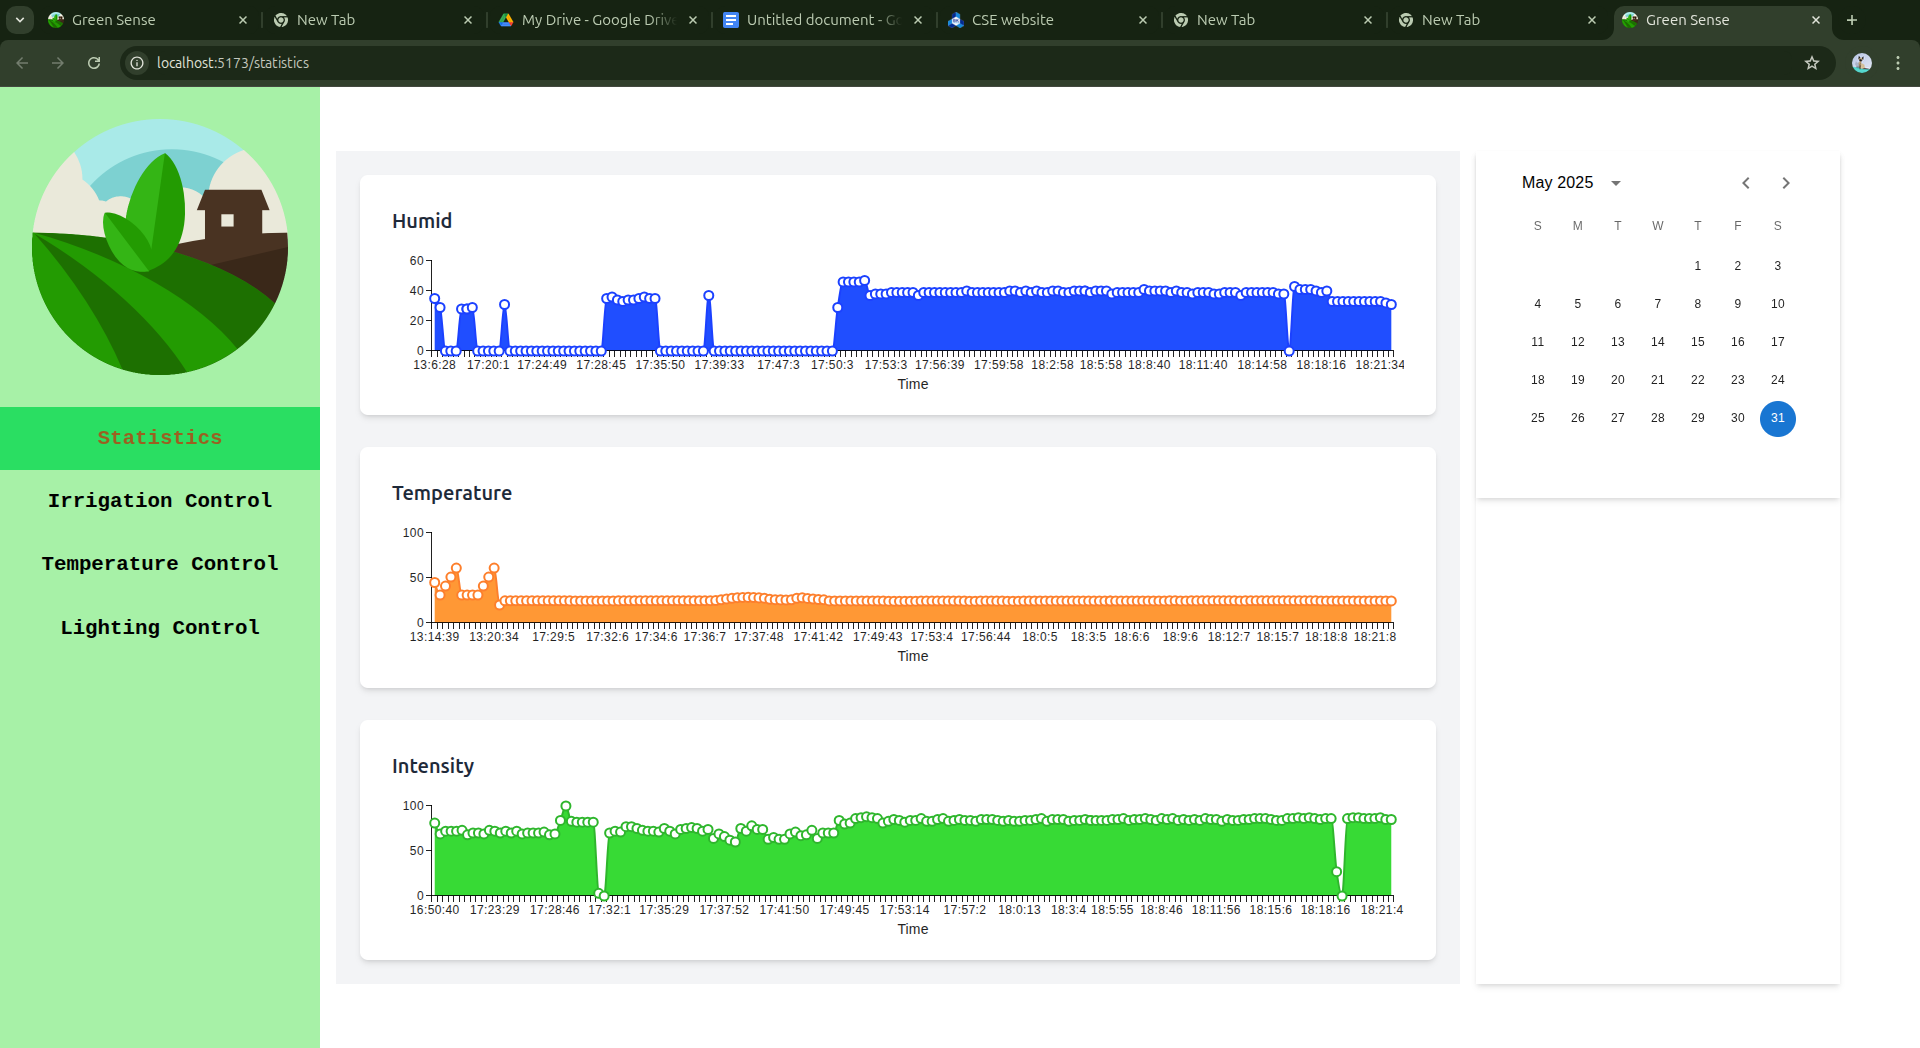
\includegraphics[width=1\linewidth]{content/images/statistics.png}
    \caption{Màn hình tính năng Dashboard}
\end{figure}

\begin{figure}[H]
    \centering
    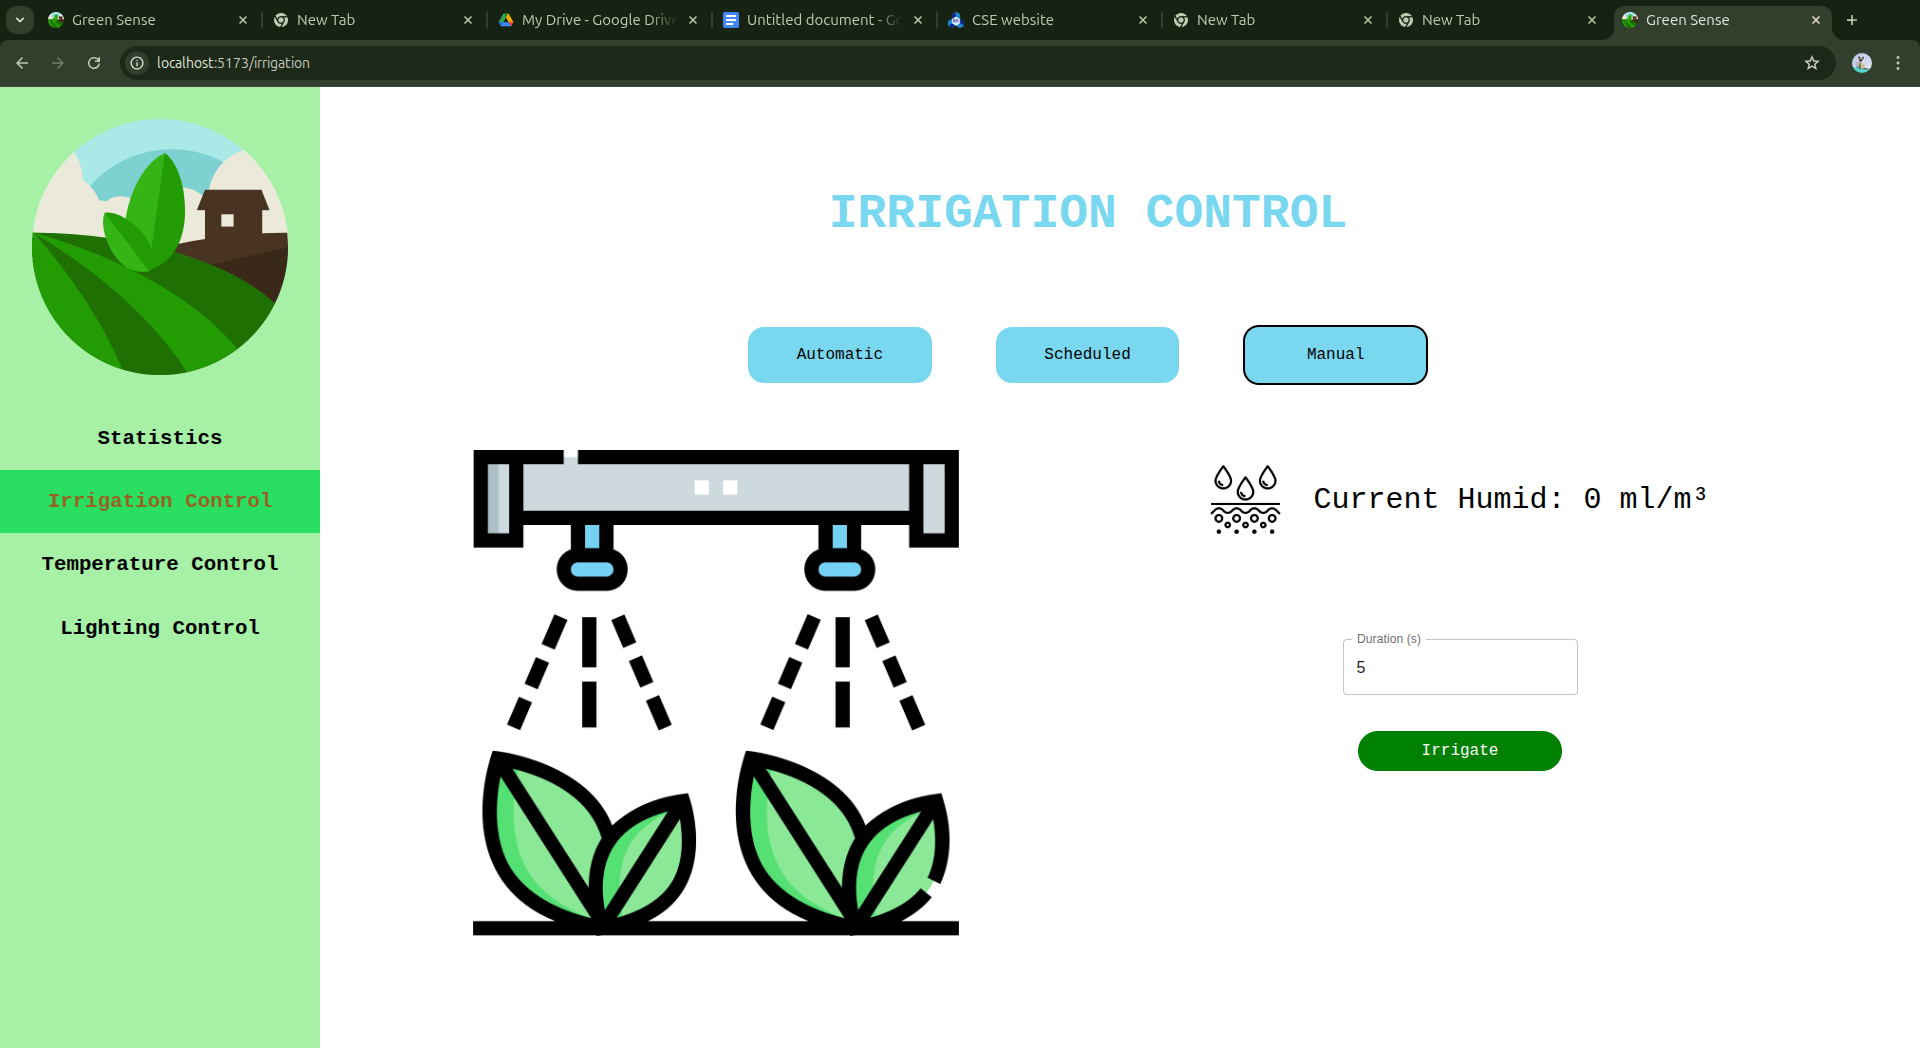
\includegraphics[width=1\linewidth]{content/images/pump_manual.png}
    \caption{Màn hình điều khiển máy bơm nước thủ công}
\end{figure}

\begin{figure}[H]
    \centering
    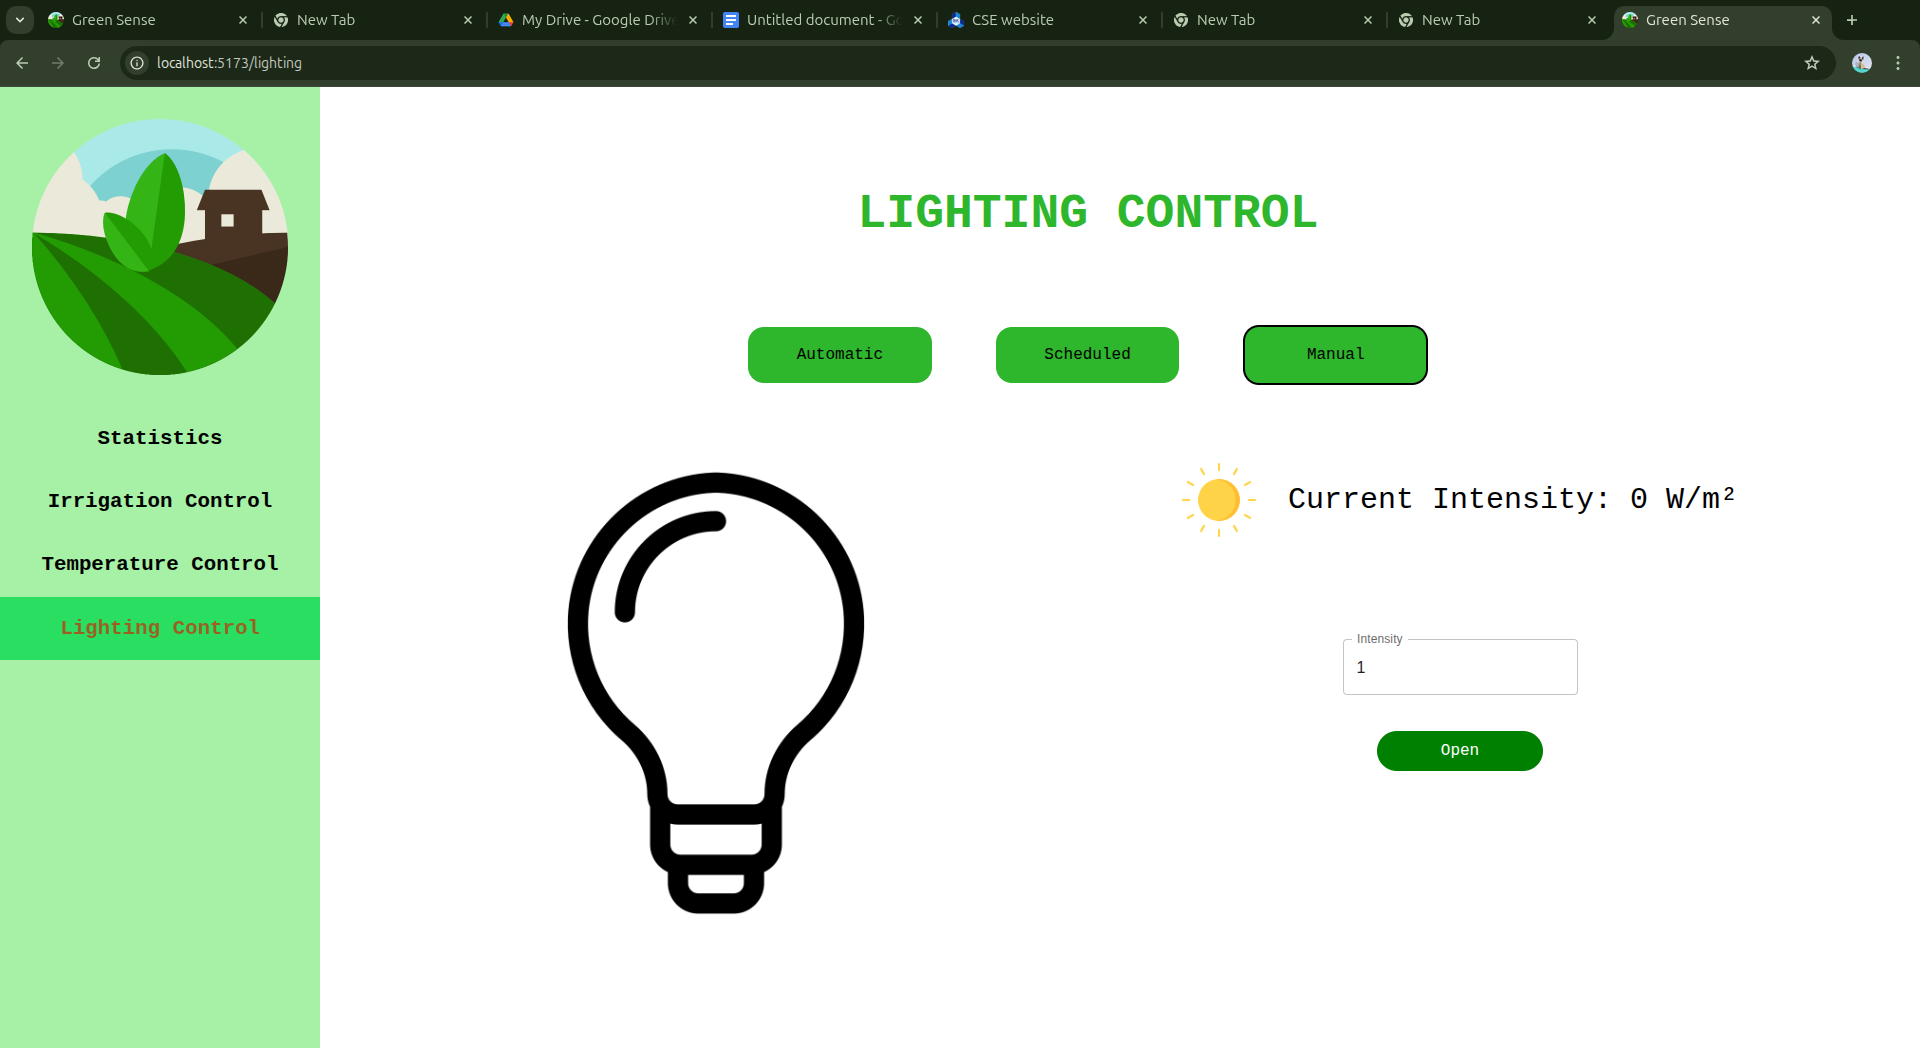
\includegraphics[width=1\linewidth]{content/images/light_manual.png}
    \caption{Màn hình điều khiển đèn thủ công}
\end{figure}

\begin{figure}[H]
    \centering
    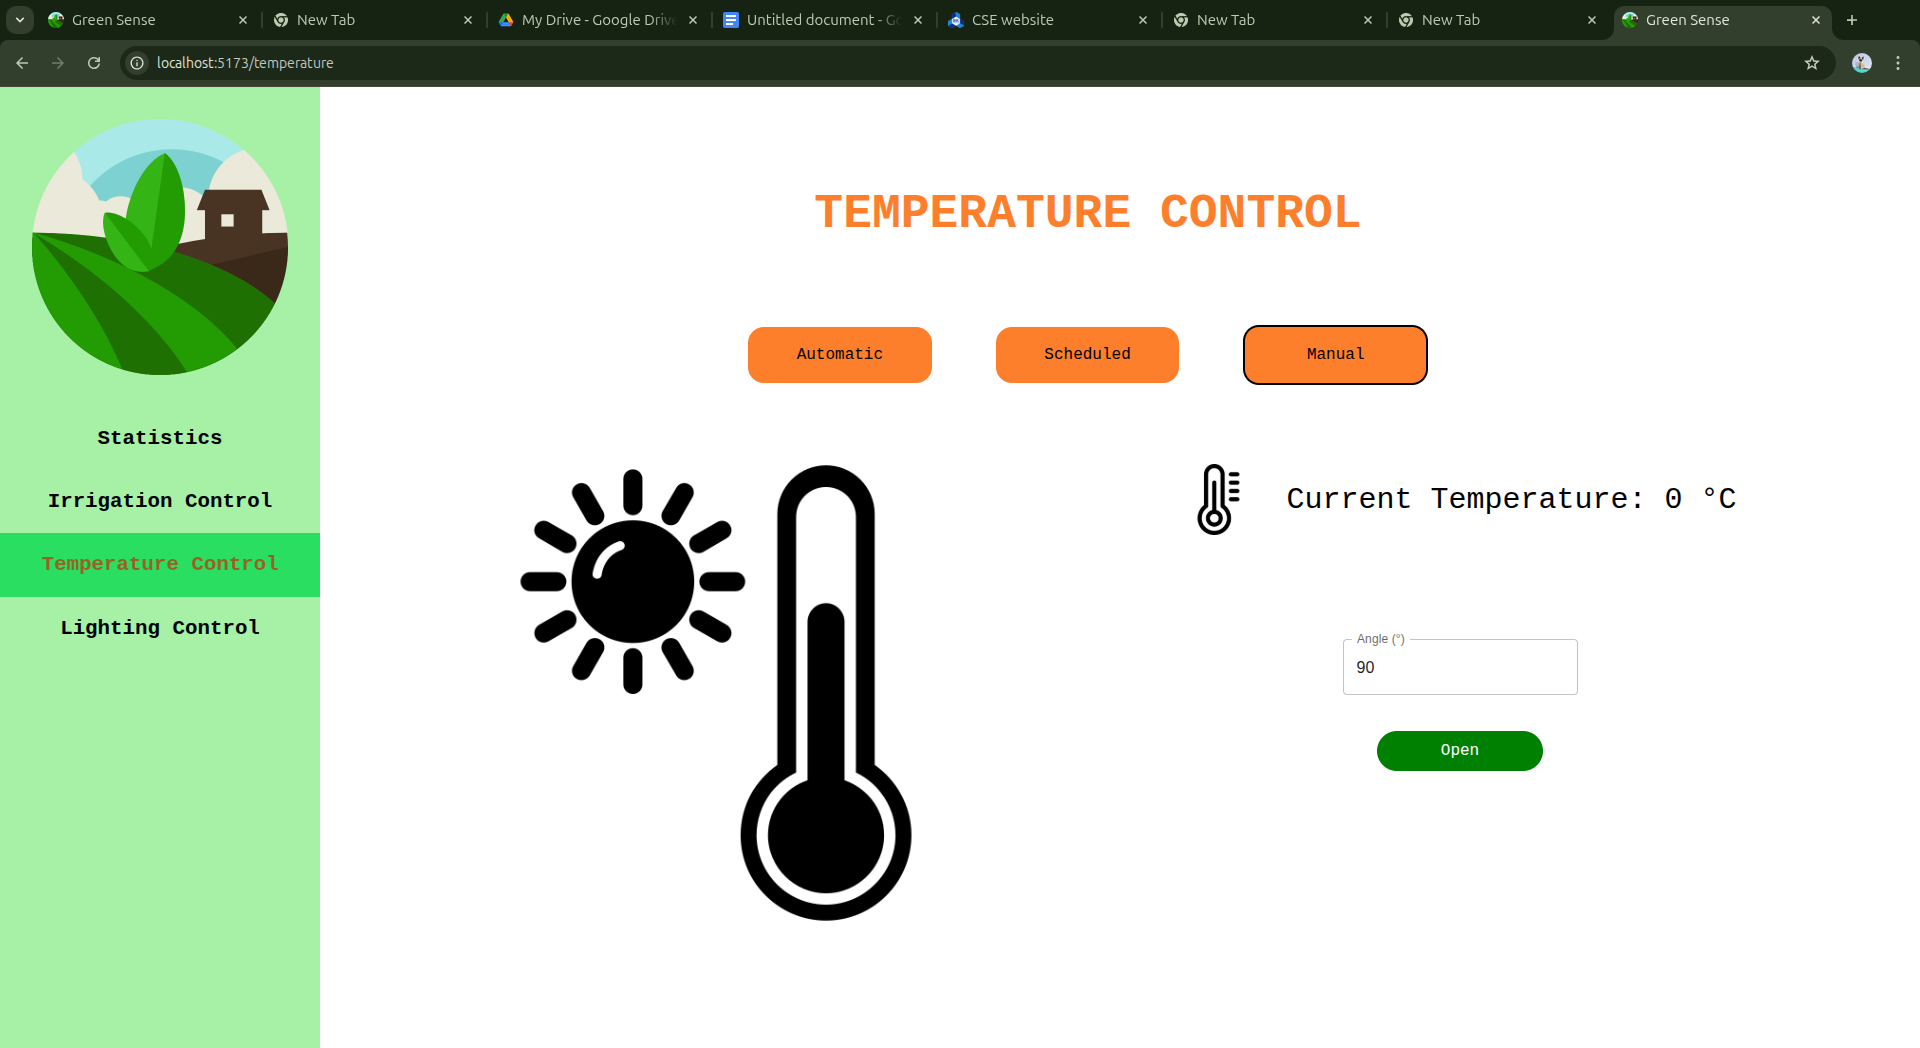
\includegraphics[width=1\linewidth]{content/images/temp_manual.png}
    \caption{Màn hình điều khiển màn che (động cơ servo) thủ công}
\end{figure}

\begin{figure}[H]
    \centering
    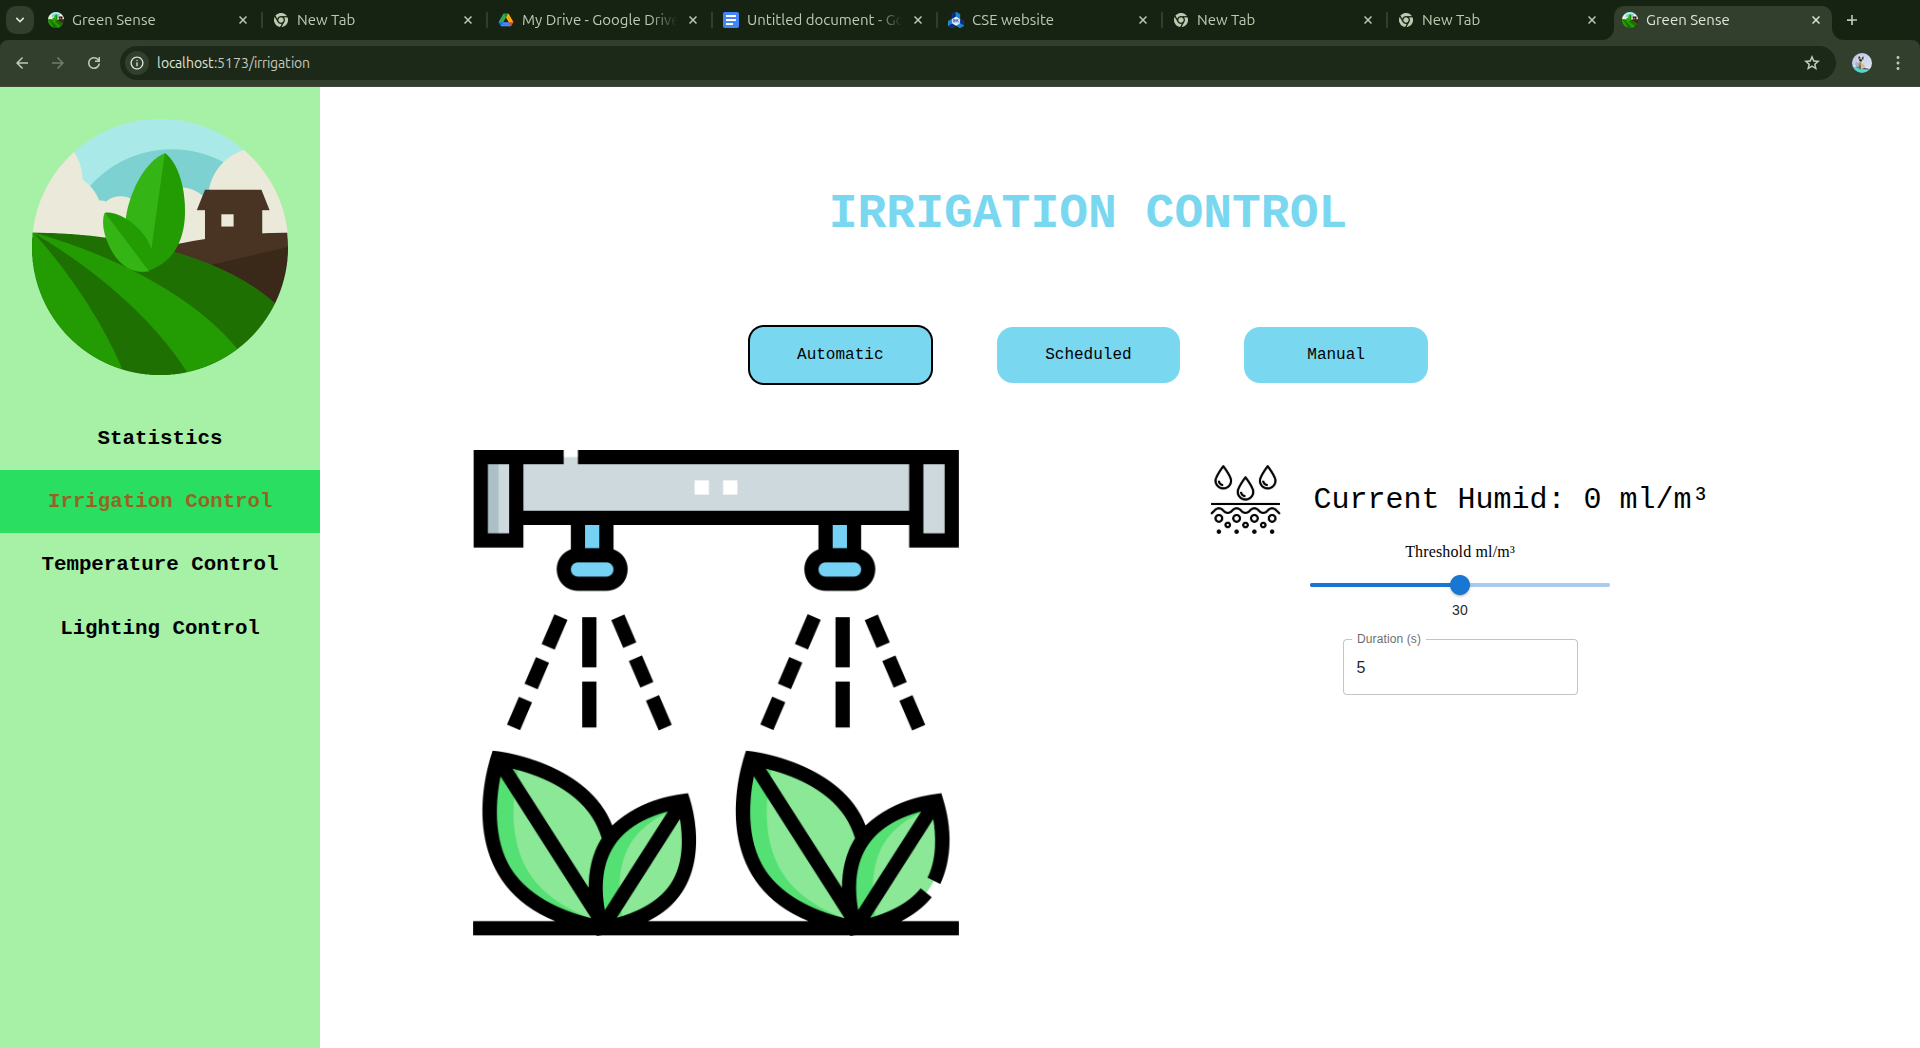
\includegraphics[width=1\linewidth]{content/images/pump_automatic.png}
    \caption{Màn hình cài đặt điều khiển máy bơm nước tự động}
\end{figure}

\begin{figure}[H]
    \centering
    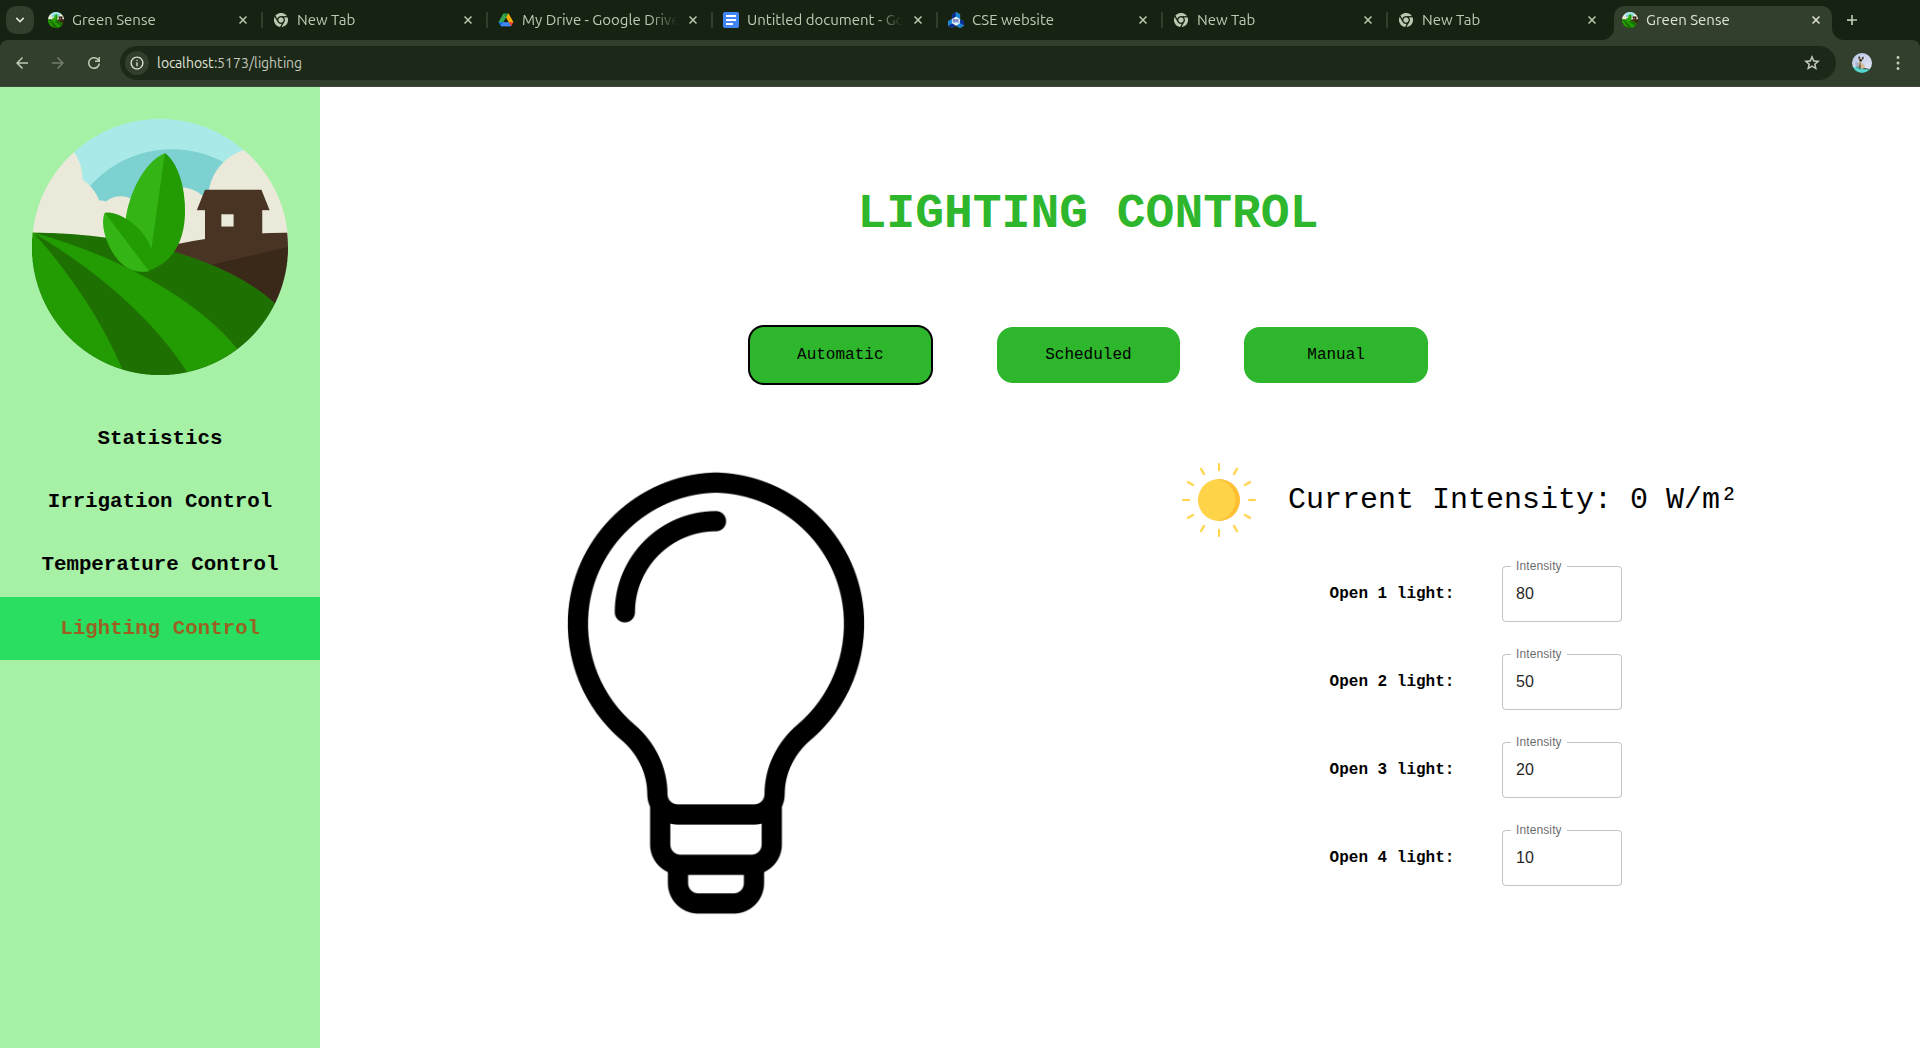
\includegraphics[width=1\linewidth]{content/images/light_automatic.png}
    \caption{Màn hình cài đặt điều khiển đèn tự động}
\end{figure}

\begin{figure}[H]
    \centering
    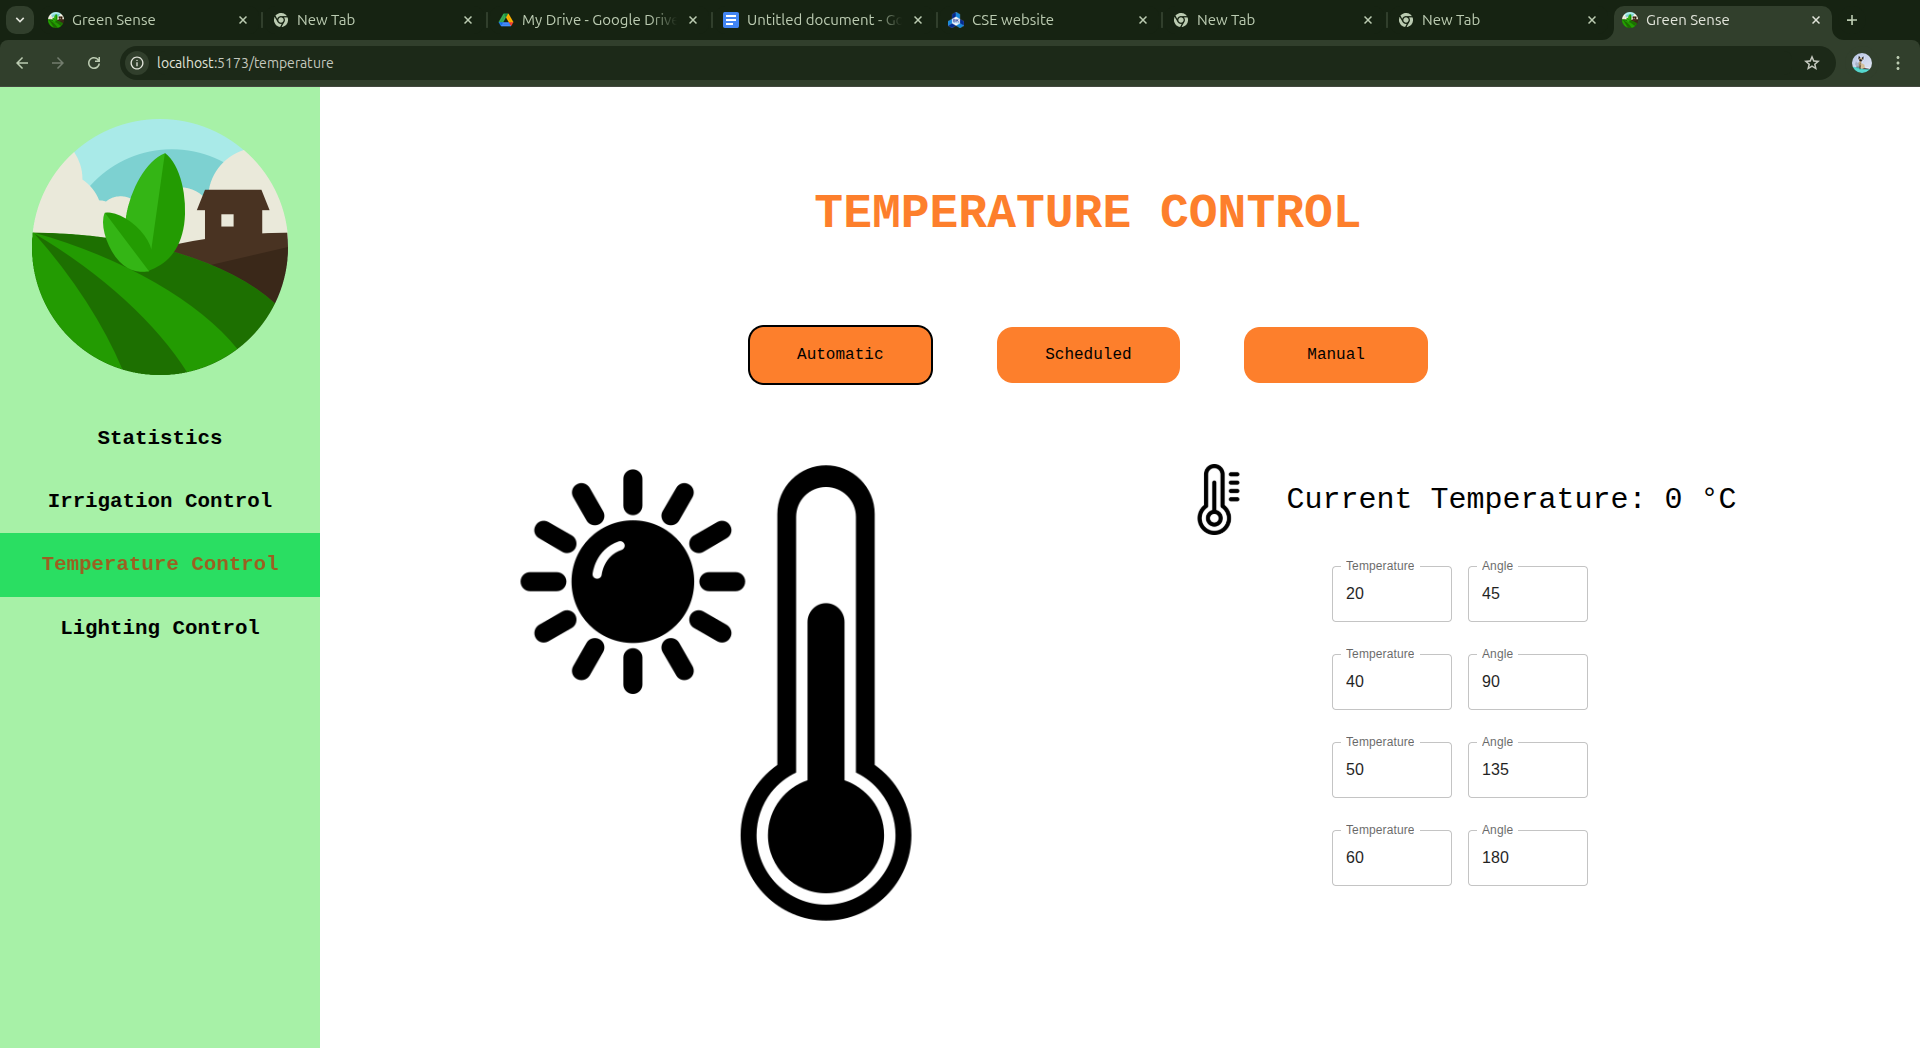
\includegraphics[width=1\linewidth]{content/images/temp_automatic.png}
    \caption{Màn hình cài đặt điều khiển màn che (động cơ servo) tự động}
\end{figure}

\begin{figure}[H]
    \centering
    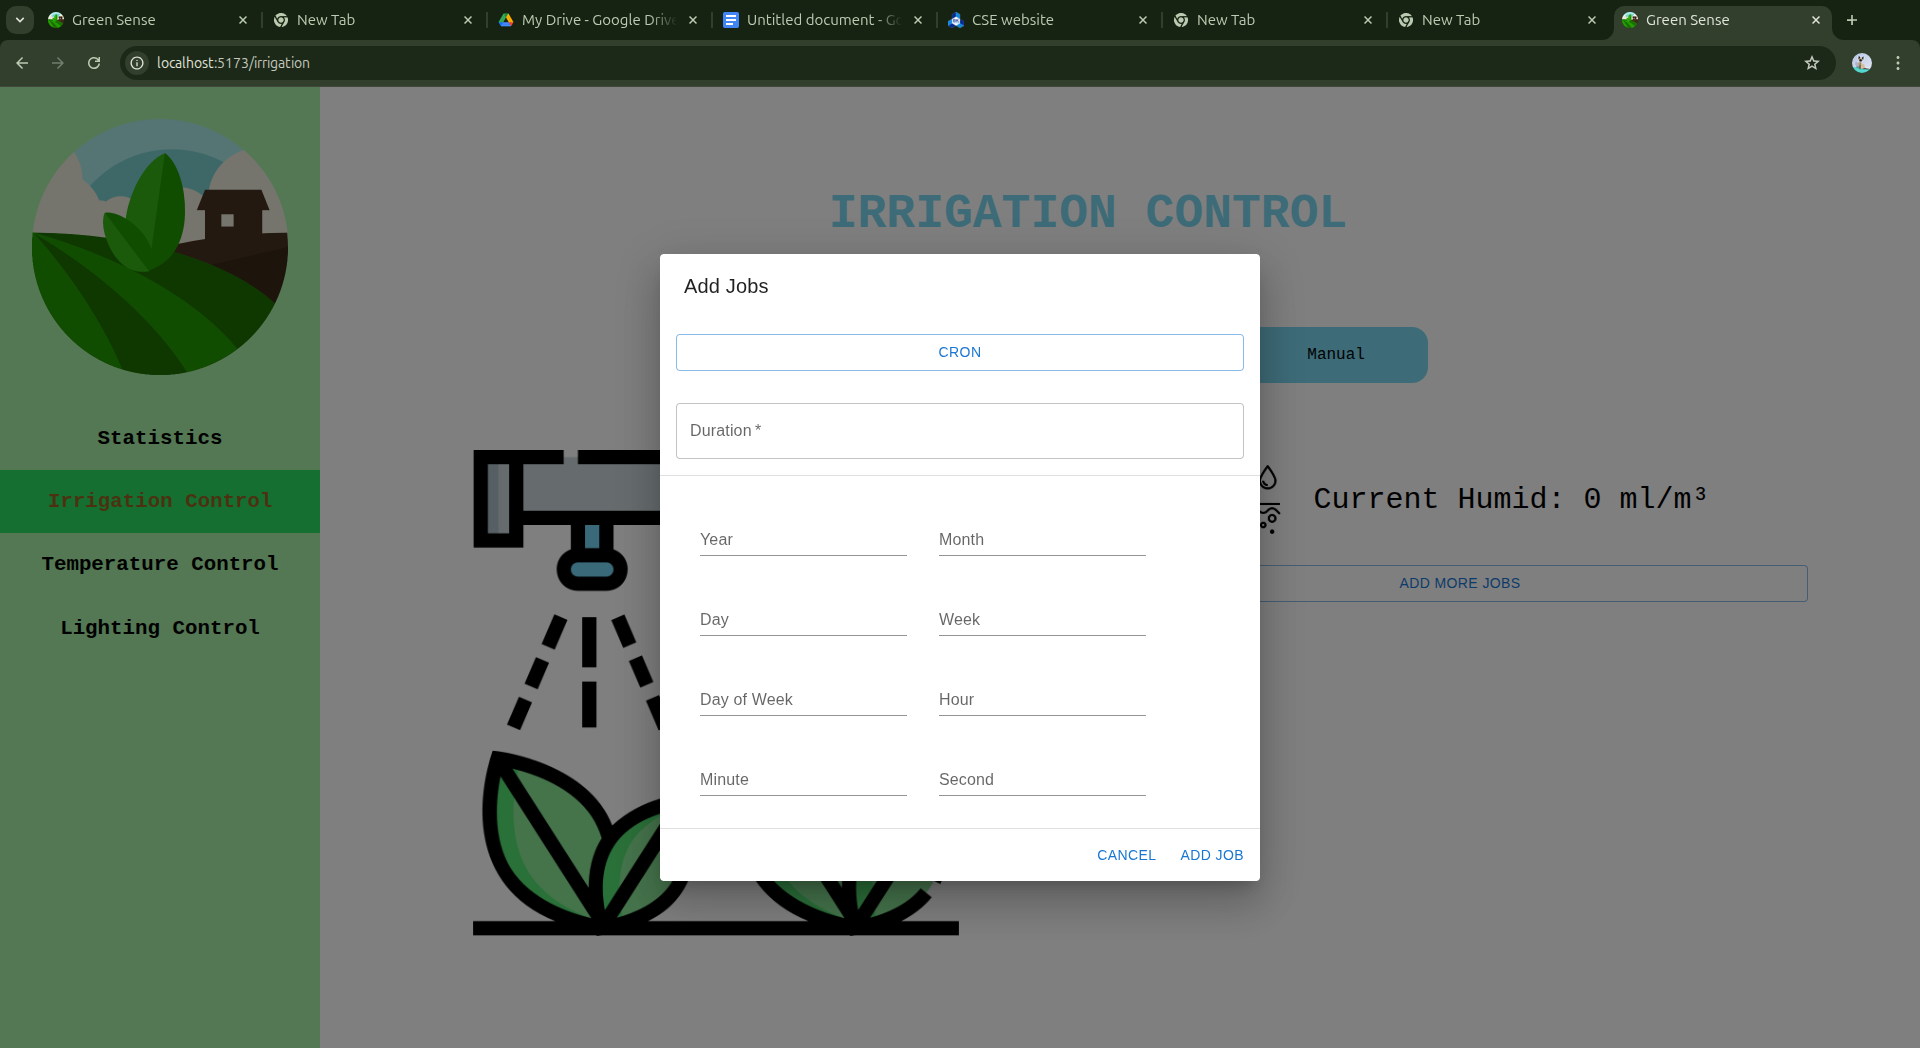
\includegraphics[width=1\linewidth]{content/images/pump_job_cron.png}
    \caption{Màn hình đặt lịch hoạt động cho máy bơm nước - theo chế độ cron}
\end{figure}

\begin{figure}[H]
    \centering
    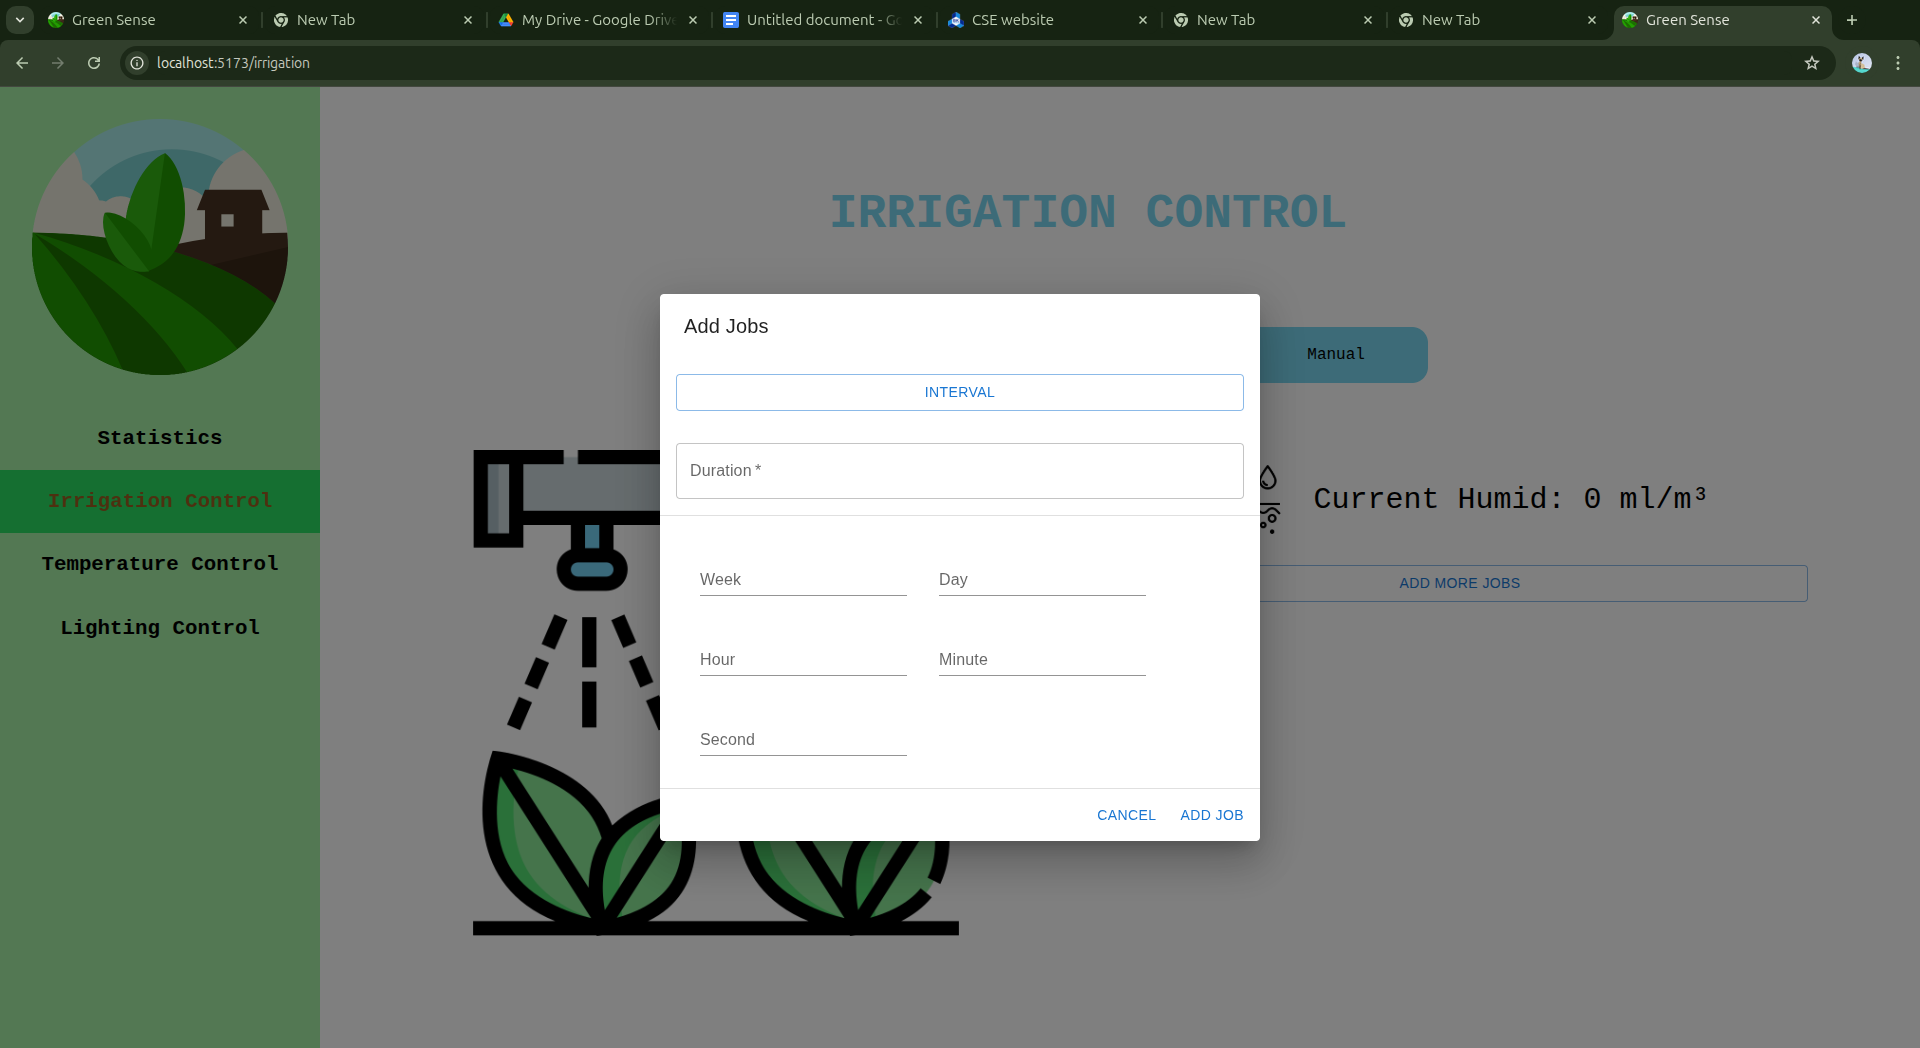
\includegraphics[width=1\linewidth]{content/images/pump_job_interval.png}
    \caption{Màn hình đặt lịch hoạt động cho máy bơm nước - theo chế độ interval}
\end{figure}

\begin{figure}[H]
    \centering
    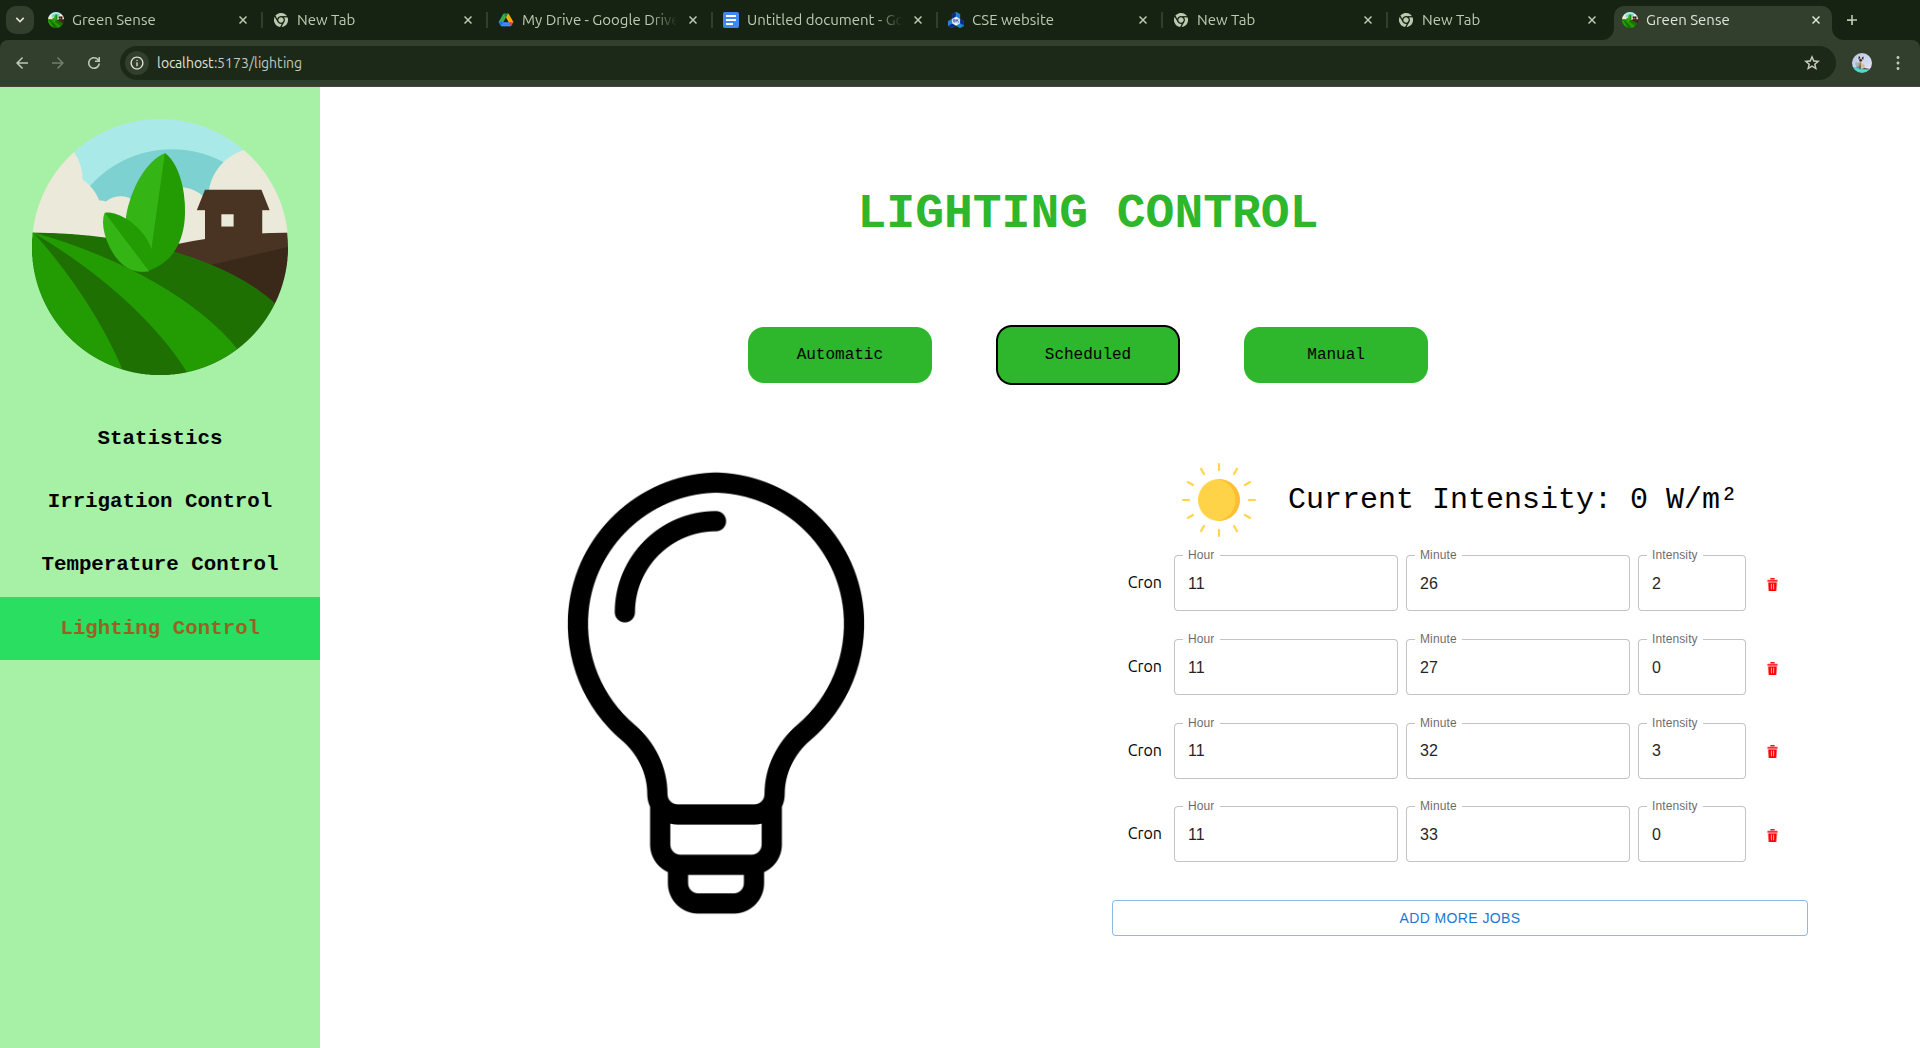
\includegraphics[width=1\linewidth]{content/images/light_job.png}
    \caption{Màn hình đặt lịch hoạt động cho đèn}
\end{figure}

\begin{figure}[H]
    \centering
    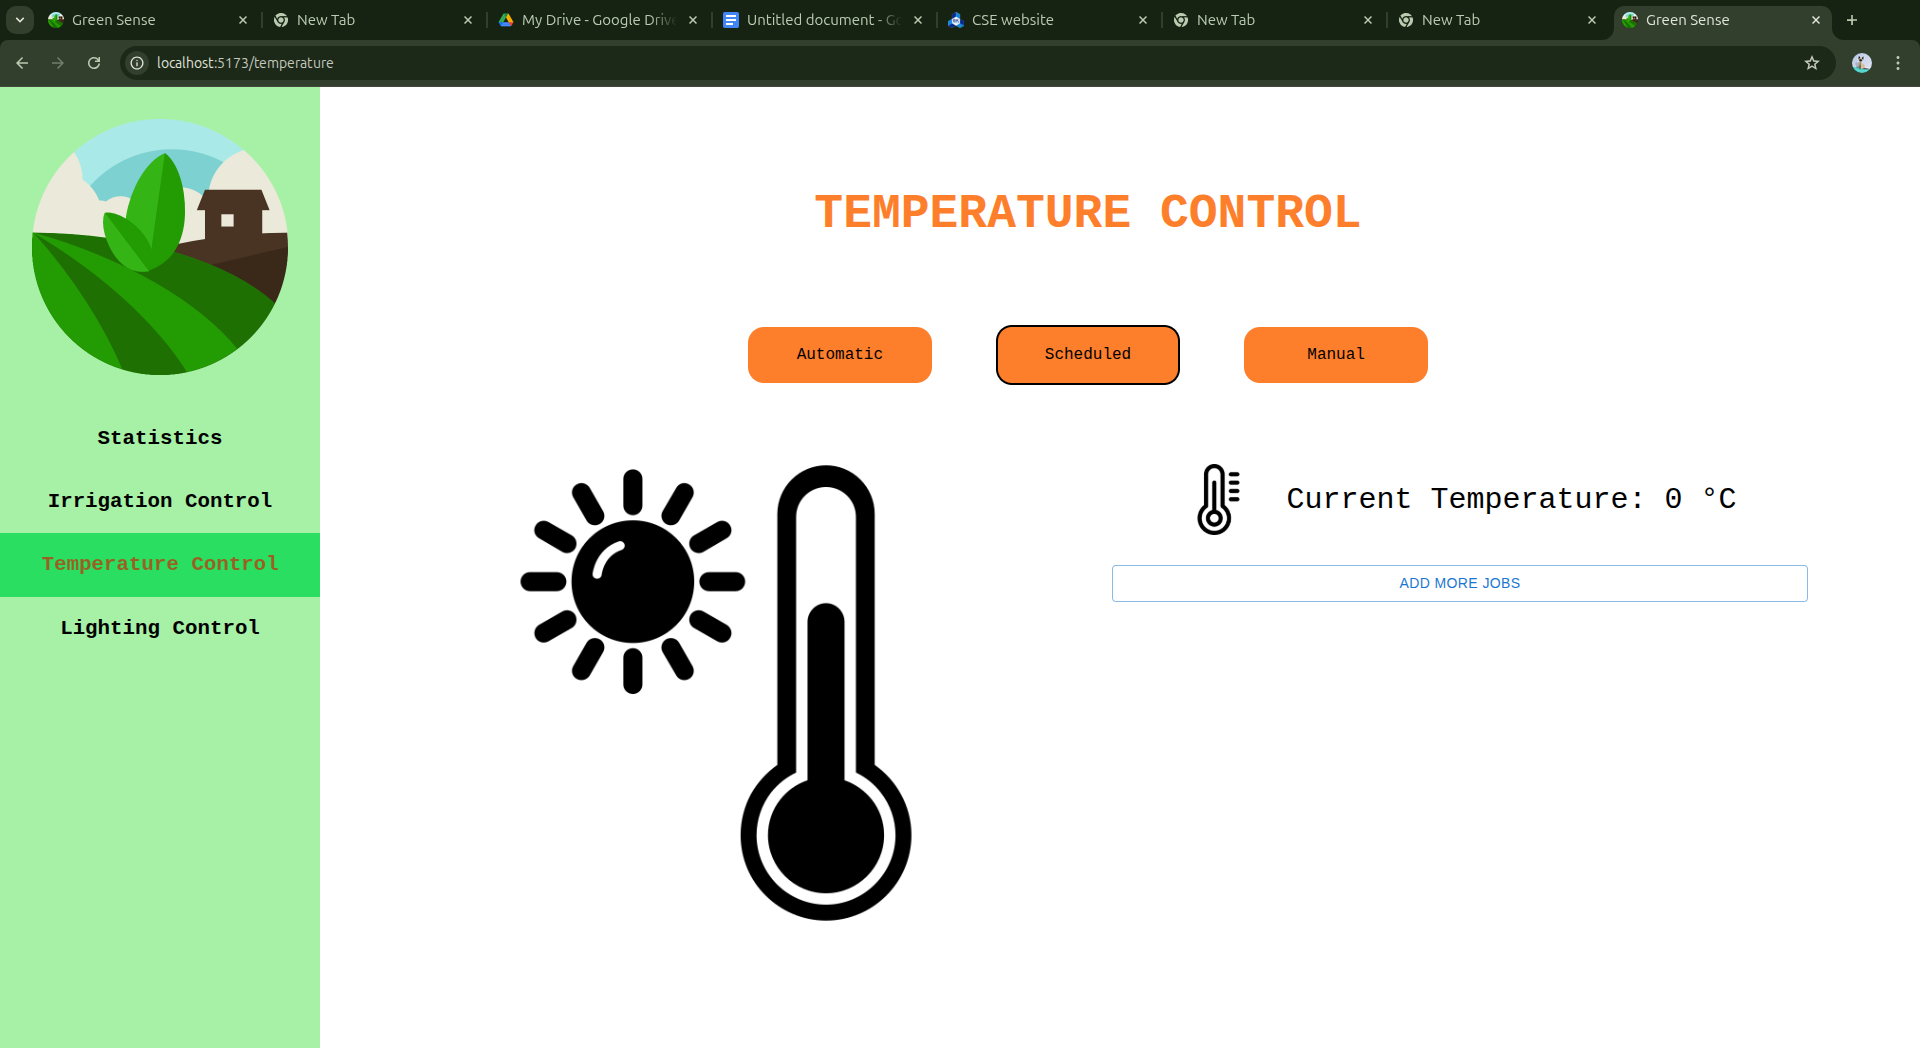
\includegraphics[width=1\linewidth]{content/images/temp_job.png}
    \caption{Màn hình đặt lịch hoạt động cho màn che (động cơ servo)}
\end{figure}

\begin{figure}[H]
    \centering
    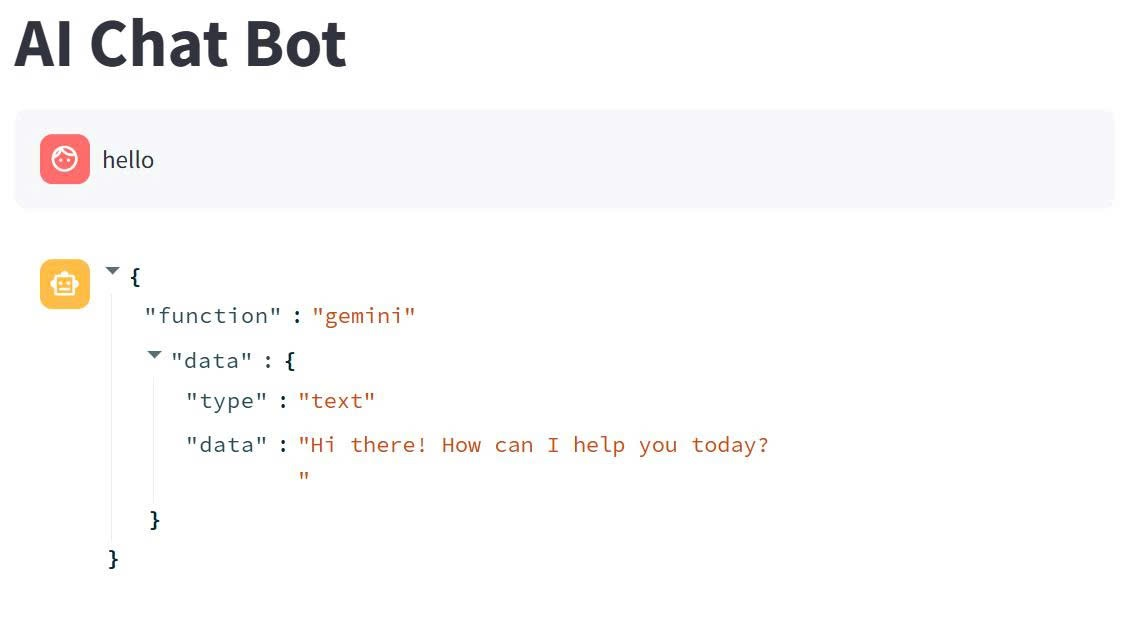
\includegraphics[width=1\linewidth]{content/images/AI_Chatbox_1.jpg}
    \caption{Màn hình khởi động AI Chatbot}
\end{figure}

\begin{figure}[H]
    \centering
    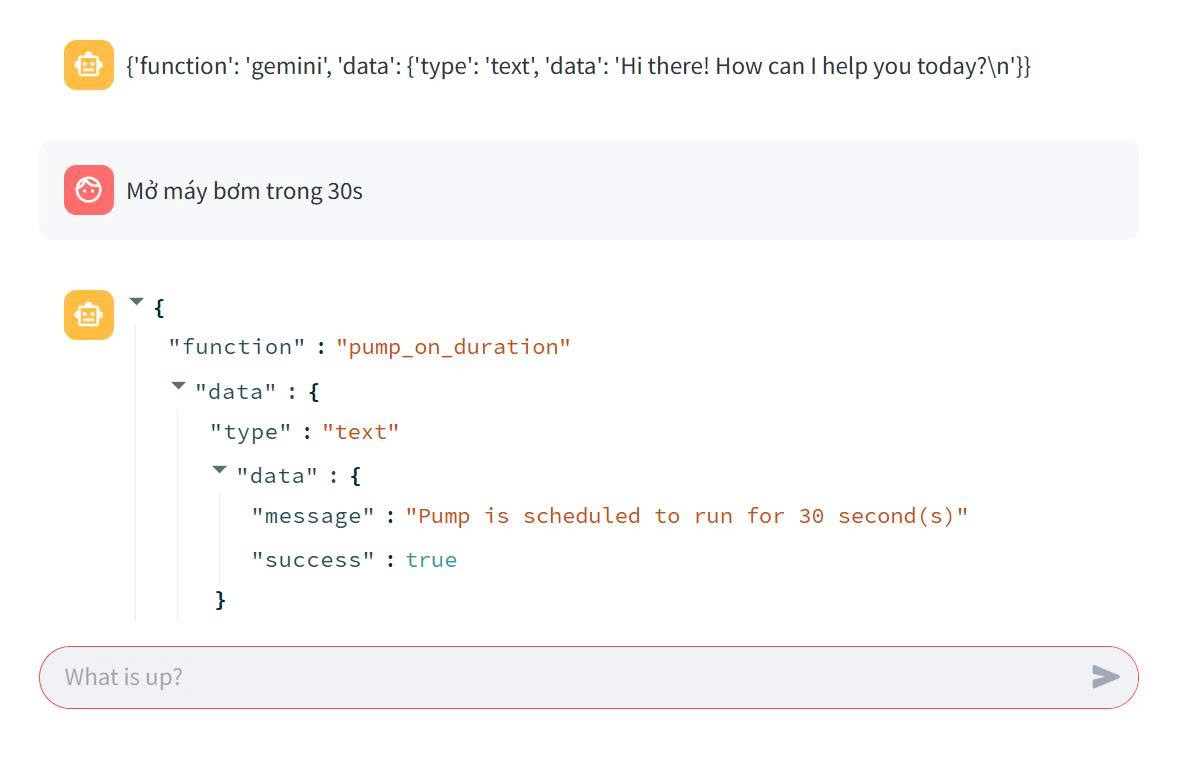
\includegraphics[width=1\linewidth]{content/images/AI_Chatbox_2.jpg}
    \caption{Điều khiển máy bơm (pump) bằng ngôn ngữ tự nhiên}
\end{figure}

\begin{figure}[H]
    \centering
    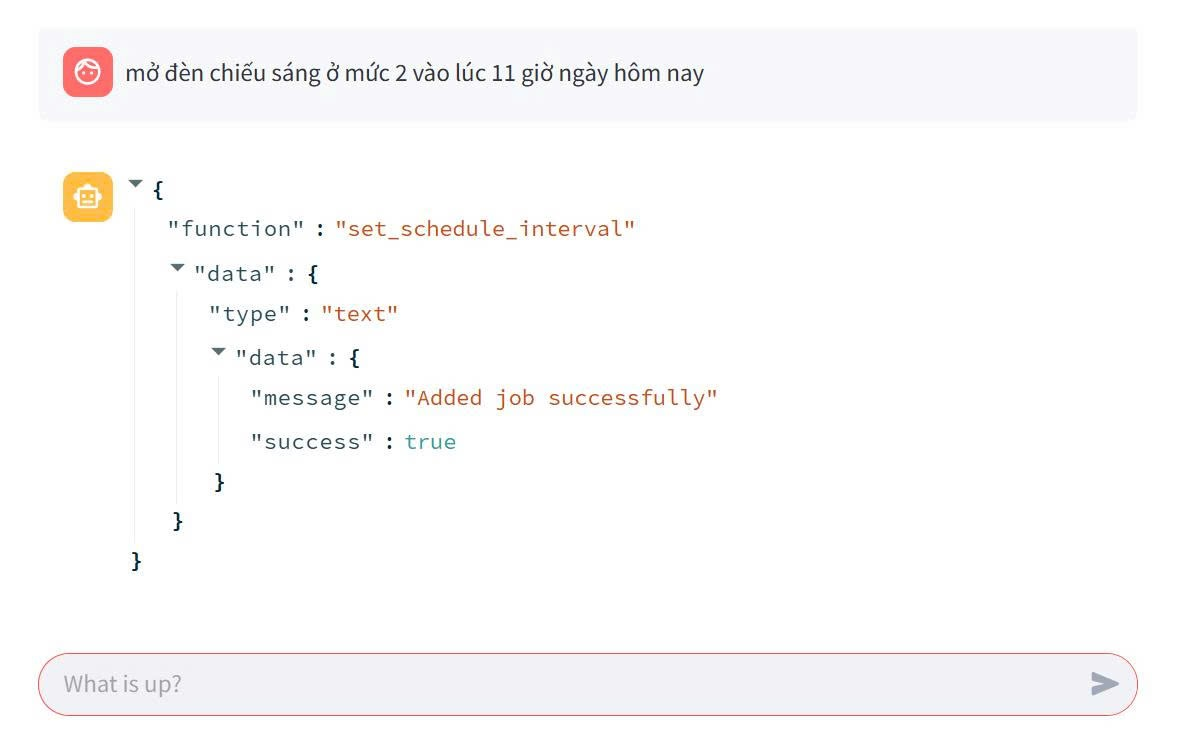
\includegraphics[width=1\linewidth]{content/images/AI_Chatbox_3.jpg}
    \caption{Đặt lịch mở đèn bằng ngôn ngữ tự nhiên}
\end{figure}

\begin{figure}[H]
    \centering
    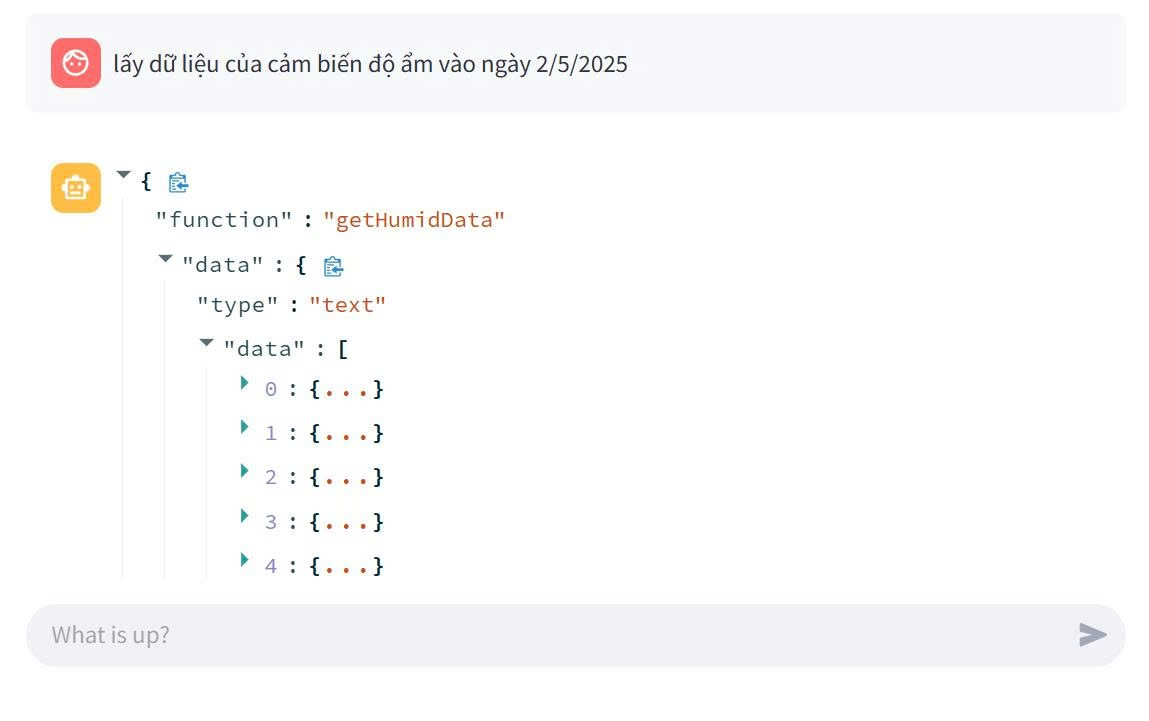
\includegraphics[width=1\linewidth]{content/images/AI_Chatbox_4.jpg}
    \caption{Lấy dữ liệu của cảm biến độ ẩm đất bằng ngôn ngữ tự nhiên}
\end{figure}

\newpage
